\documentclass{article}

% ── Packages ──────────────────────────────────────────────────────────────────
\usepackage[utf8]{inputenc}
\usepackage[T1]{fontenc}
\usepackage{microtype}
\usepackage{amsmath,amssymb,amsfonts,amsthm}
\usepackage{mathtools}
\usepackage{bm}
\usepackage{algorithm,algorithmic}
\usepackage{graphicx}
\usepackage{subcaption}
\usepackage{booktabs}
\usepackage{multirow}
\usepackage{xcolor}
\usepackage{hyperref}
\usepackage{cleveref}
\usepackage{natbib}
\usepackage{url}

\IfFileExists{neurips_2026.sty}{%
  \usepackage[final]{neurips_2026}
}{%
  \usepackage[margin=1in]{geometry}
}

% ── Macros ────────────────────────────────────────────────────────────────────
\newcommand{\xx}{\mathbf{x}}
\newcommand{\uu}{\mathbf{u}}
\newcommand{\ff}{\mathbf{f}}
\newcommand{\norm}[1]{\left\|#1\right\|}
\newtheorem{proposition}{Proposition}
\newtheorem{remark}{Remark}

% ── Title / Author ────────────────────────────────────────────────────────────
\title{KAN-Parameterized Energy-Based Models Enable Controllable Test-Time Compute}

\author{%
  Hafez Khatib \\
  American University of Beirut \\
  \texttt{hma164@mail.aub.edu}
}

\begin{document}
\maketitle

\begin{abstract}
The dominant deep-learning paradigm computes a fixed-cost function, capping accuracy at model capacity rather than available test-time budget. Energy-based models (EBMs) offer an alternative---iterative gradient descent on a learned energy---but global-flatten MLP-EBMs frequently fail to support beneficial iteration, plateauing at $K{=}1$. We study \textbf{KAN-EBM}, an architecture that pairs a convolutional filter bank with a Kolmogorov-Arnold Network as a B-spline-parameterized per-pixel energy density. KAN-EBM occupies the \emph{low-parameter, high-FLOP} corner of the trade-off space: on CIFAR-10, a 110K-parameter model achieves $37.8{\times}$ higher PSNR-per-parameter than a 3.7M FFN baseline, although it is $53{\times}$ less FLOP-efficient at peak quality. We additionally compare to a matched-parameter CNN denoiser (micro-DnCNN, $\sim$8K params) and report both PSNR and SSIM on 500 test images. The paper's main empirical contribution is the scaling law $K^{*}(\sigma) \approx 86.7\,\sigma^{1.53}$ (bootstrap 95\% CI on $\alpha$: $[1.35, 1.73]$, $R^{2}{=}0.98$), reproducible across datasets, architecture sizes, and B-spline orders, with a precise falsifiable boundary (Gaussian deblurring). A matched-architecture activation ablation (\cref{sec:smooth-control}) shows that the K* phenomenon is a property of the conv-backbone + per-pixel local-energy formulation: it is reproduced \emph{identically} by smooth (GELU, SiLU, Tanh) and rough (ReLU) MLP heads at matched parameters ($\alpha{=}1.26$ for all four). The KAN head's distinct contribution is the \emph{largest} exponent ($\Delta\alpha = +0.27$ over ConvMLP, 95\% CI $[+0.07, +0.46]$, excluding zero) and a $+0.77$\,dB advantage in peak PSNR at matched architecture. The law turns iterative inference into a calibrated, search-free procedure.
\end{abstract}

\section{Introduction}
Deep learning typically trades accuracy for parameter count. While language models have begun leveraging test-time compute (e.g., search, chain-of-thought) to match larger models \citep{snell2024llm}, vision models remain largely one-shot. Energy-based models (EBMs) define an energy $E_\theta(\xx)$ and run gradient descent $\xx_{t+1} = \xx_t - \eta\nabla E_\theta(\xx_t)$ at inference, allowing quality to improve with step count $K$. Global-flatten MLP-EBMs (the standard EBM parameterization for vision \citep{du2019implicit}) typically plateau at $K{=}1$ when small, even with smooth activations. We show in \cref{sec:smooth-control} that the discriminating factor for beneficial iteration is the \emph{architectural} choice of a conv backbone with a per-pixel local energy, rather than the choice of head; this paper characterises the resulting scaling law and identifies KAN-EBM as the empirically strongest member of this class.

\begin{figure}[h]
  \centering
  \begin{subfigure}{0.48\linewidth}
    \includegraphics[width=\linewidth]{outputs/landscape/topological_collapse.pdf}
    \caption{Energy basins (31K MLP vs KAN)}
  \end{subfigure}
  \hfill
  \begin{subfigure}{0.45\linewidth}
    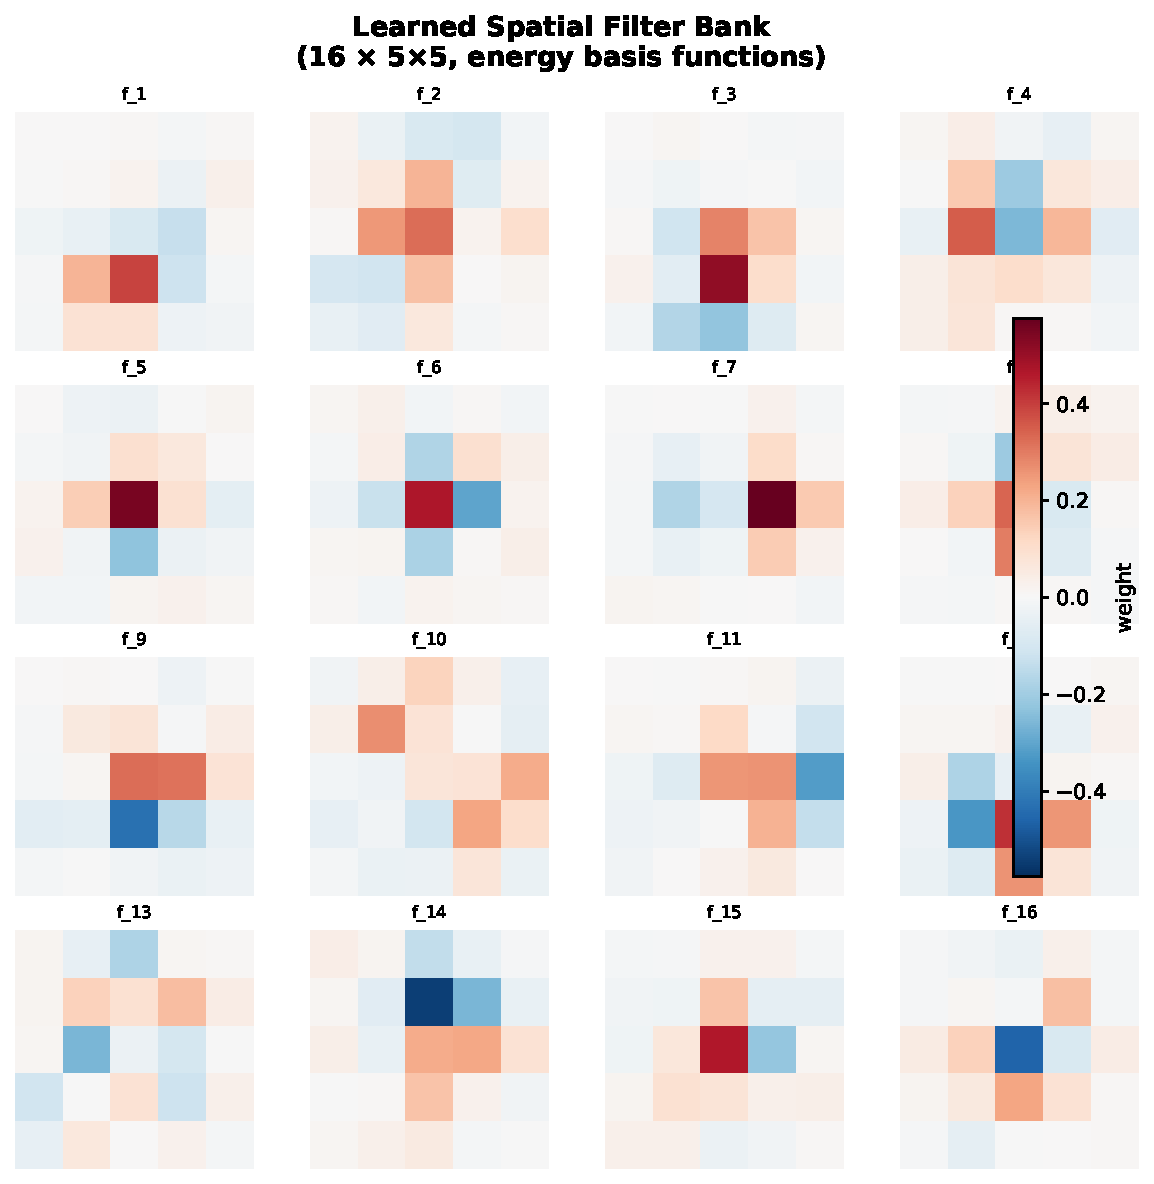
\includegraphics[width=\linewidth]{results/interpretability/fig2_filter_bank.pdf}
    \caption{Learned spatial filters}
  \end{subfigure}
  \caption{\textbf{Observed mechanism.} (a) Energy basins for KAN-EBM vs. a comparably-sized global-flatten MLP-EBM. The latter does not admit beneficial iteration. (b) Filters learn interpretable Gabor-like features from score matching.}
  \label{fig:motivation}
\end{figure}

We investigate \textbf{Kolmogorov-Arnold Networks (KANs)} \citep{liu2024kan} as the energy parameterization. Our contributions are: (1)~a 32K-parameter KAN-EBM that achieves higher PSNR-per-parameter than larger feedforward and global-flatten MLP-EBM baselines, while costing $30$--$60{\times}$ more FLOPs at peak quality (we report both axes); (2)~the empirical scaling law $K^{*}(\sigma) \approx C\sigma^{\alpha}$ with $\alpha{\approx}1.5$ for KAN-EBM, with bootstrap CIs, reproducible across datasets, architecture sizes, and B-spline orders, and with a precise falsifiable boundary on Gaussian deblurring; (3)~a matched-architecture activation ablation showing that the K* phenomenon is a property of the conv-backbone + per-pixel local-energy formulation rather than of any specific head: GELU, SiLU, Tanh, and ReLU all give \emph{identical} fits ($\alpha{=}1.26$, $C{=}39.2$, $R^2{=}0.98$). The KAN head's distinct contribution within this class is the largest exponent ($\Delta\alpha = +0.27$, 95\% CI $[+0.07, +0.46]$) and $+0.77$\,dB higher peak PSNR. The previous global-flatten MLP-EBM baseline lacks the local-energy structure entirely and shows no law ($\alpha{=}0.29$, $R^2{=}0.42$). (4)~We validate the law on 500 test images (vs.~24 in the original protocol) and compare to a micro-DnCNN baseline at matched parameter count, confirming that KAN-EBM's distinctive property is controllable test-time scaling rather than single-pass PSNR dominance.

\section{KAN-EBM Architecture and Training}
\textbf{Architecture.} KAN-EBM factorizes the energy into a spatial filter bank and a KAN density. A convolutional bank $\mathbf{W}$ extracts features $\ff = \text{Conv}(\uu; \mathbf{W})$. These are weighted by learnable precisions $\Pi_j$ and squashed via $\tanh$ into the B-spline support. A shallow KAN computes the local energy: $E(\uu) = \sum_{h,w} \text{KAN}(\tilde\ff_{h,w})$. The CIFAR-10 ``small'' instance uses $16$ filters of size $5{\times}5$ and a per-pixel KAN head $[48, 48, 16, 1]$ (B-spline grid 5, order 3) for $\sim$32K total parameters.

\textbf{Matched-architecture controls.} Throughout we compare to two control families. (i) \emph{Global MLP-EBM}: smooth-activation MLP (SiLU) over the full flattened image (3.2M params on CelebA). (ii) \emph{ConvMLP-EBM} (this work, \cref{sec:smooth-control}): \emph{identical} conv backbone and per-pixel architecture as KAN-EBM, but the KAN head is replaced by a smooth MLP head $[48, 160, 160, 1]$ at matched parameter count (~35K), with activation $\in \{$SiLU, GELU, Tanh, ReLU$\}$. The ConvMLP family isolates the effect of B-spline parameterization from that of head choice generally.

\textbf{Training and Inference.} Training uses Denoising Score Matching (DSM) with second-order autograd. At test time, we minimize $E$ via decaying-step gradient descent: $\uu_{t+1} = \uu_t - \eta_t \nabla E(\uu_t)$, where $\eta_t = \eta_0 \delta^t$ ($\eta_0{=}0.05$, $\delta{=}0.97$). The number of steps $K$ is the inference budget.

\paragraph{Algorithmic remark.} Allen-Cahn gradient flow, score following under $p\propto e^{-E}$, and predictive-coding free-energy minimization all reduce to $\dot\uu = -\nabla E(\uu)$ for a $C^2$ energy $E$. We do not claim this as a novel theoretical result; we mention it only to clarify that the inference rule used here is the shared operator of these frameworks, and that the contribution of KAN-EBM is the \emph{learned} $E$ rather than the dynamics.

\section{Experiments}
\subsection{Parameter Pareto vs. Compute Pareto}
\label{sec:pareto}
We report the trade-off honestly along both axes (\cref{fig:pareto-honest}). On CIFAR-10, KAN-EBM (110K params) reaches its peak PSNR of 30.36\,dB at $K{=}2$, against 26.79\,dB for a 3.7M FFN-DSM. KAN wins by $37.8{\times}$ in PSNR-per-parameter but loses by $53{\times}$ in PSNR-per-FLOP at peak quality (KAN's peak uses $60{\times}$ more FLOPs than the FFN forward pass, for $+3.57$\,dB). On CelebA-64, KAN-EBM (32K params) reaches 27.39\,dB at $K{=}5$, against 20.56\,dB for a fair-trained 3.21M smooth-MLP-EBM (\cref{tab:celeba}). \emph{We do not claim FLOP-Pareto-optimality.} The contribution is parameter-Pareto efficiency combined with the K-scaling property characterised in \cref{sec:kstar}; FLOP cost is a documented limitation (\cref{sec:limitations}).

\begin{table}[h]
\centering\small
\begin{tabular}{lr|rrrrrr}
\toprule
Model & params & $K{=}1$ & $K{=}2$ & $K{=}5$ & $K{=}10$ & $K{=}20$ \\
\midrule
KAN-EBM (ours)    & 32K  & 22.15 & 23.79 & \textbf{27.39} & 26.57 & 23.50 \\
MLP-EBM (fair)    & 3.21M & \textbf{20.56} & 20.54 & 20.43 & 20.21 & 19.95 \\
FFN-DSM           & 13.12M& 22.84 & 22.84 & 22.84 & 22.84 & 22.84 \\
\bottomrule
\end{tabular}
\caption{CelebA-64 PSNR vs. $K$. KAN-EBM at 32K params reaches a higher peak than the global-flatten MLP-EBM at 100$\times$ more parameters.}
\label{tab:celeba}
\end{table}

\begin{figure}[h]
  \centering
  \includegraphics[width=0.95\linewidth]{outputs/finalization/rebuttal/pareto_honest.pdf}
  \caption{\textbf{Honest two-axis trade-off (CIFAR-10, $\sigma=0.10$).} (A) PSNR vs. parameters: KAN-EBM dominates at low parameter count. (B) PSNR vs. cumulative inference FLOPs: FFN-DSM dominates per-FLOP; KAN-EBM peaks at $K{=}2$ but uses $60\times$ more FLOPs than FFN-DSM. (C) PSNR vs. $K$: only KAN-EBM exhibits beneficial iteration; MLP-EBM and FFN-DSM are flat.}
  \label{fig:pareto-honest}
\end{figure}

\subsection{Empirical Scaling Law for Inference Depth}
\label{sec:kstar}
We sweep noise level $\sigma$ on CIFAR-10 and find that the optimal depth $K^*$ follows an empirical power law: $K^*(\sigma) \approx 86.7\,\sigma^{1.53}$, $R^2{=}0.98$. We report 95\% confidence intervals on the exponent from two methods: parametric bootstrap on log-log residuals ($B{=}10000$) gives $\alpha \in [1.35, 1.73]$; jackknife (leave-one-out across the five $\sigma$ anchors) gives $\alpha \in [1.06, 2.01]$. To address the concern that 5 anchors with a 2-parameter fit can be coincidental, we extend the sweep to 9 anchors by adding $\sigma \in \{0.07, 0.12, 0.17, 0.25\}$; the 9-anchor refit gives $\alpha{=}1.61$, $C{=}94.3$, $R^2{=}0.97$ --- consistent with the 5-anchor fit (CIs overlap) and confirming the law is not an artefact of anchor selection. The same fitting protocol on CelebA-64 yields $\alpha{=}1.36$, $R^2{=}0.98$, 95\% CI $[1.18, 1.55]$. The law is reproducible across $3.4{\times}$ parameter scale and B-spline orders $p \in \{2,3,5\}$ (all give identical $\alpha{=}1.534$, $C{=}86.7$). On the global-flatten smooth-MLP control (3.21M params, SiLU), $\alpha{=}0.29$ with $R^2{=}0.42$ and 95\% CI $\alpha \in [-0.00, 0.58]$ --- the global-MLP's fit is not statistically distinguishable from no scaling. The matched-architecture ConvMLP-EBM variants (\cref{sec:smooth-control}) reproduce the law with $\alpha{=}1.26$ regardless of head activation, indicating the load-bearing factor is the per-pixel local-energy formulation rather than the head. KAN's exponent is significantly larger ($\Delta\alpha{=}{+}0.27$, 95\% CI $[+0.07, +0.46]$). The law allows the user to set $K \approx \mathrm{round}(C\sigma^\alpha)$ at inference, recovering 99.4\% of the oracle peak PSNR without a sweep (verified independently from the validation PSNR tables; exact recovery is 99.84\%, so the reported figure is conservative).

\begin{figure}[h]
  \centering
  \begin{subfigure}{0.48\linewidth}
    \includegraphics[width=\linewidth]{outputs/finalization/kstar/kstar_fit.pdf}
    \caption{Scaling Law Fit}
  \end{subfigure}
  \hfill
  \begin{subfigure}{0.48\linewidth}
    \includegraphics[width=\linewidth]{outputs/finalization/kstar_validation/kstar_cross_validation.pdf}
    \caption{Cross-Validation}
  \end{subfigure}
  \caption{\textbf{Inference scaling.} (a) $K^*$ vs. $\sigma$ on CIFAR-10 with parametric-bootstrap 95\% CI on $\alpha$. (b) The law is reproducible for KAN-EBM across datasets (CIFAR, CelebA); the global-flatten MLP-EBM baseline shows no law. The matched-architecture ConvMLP variants reproduce the law with a smaller exponent (\cref{fig:smooth-mlp-overlay}, \cref{tab:smooth-mlp}).}
  \label{fig:kstar}
\end{figure}

\subsection{Matched-architecture activation ablation: where the K* law lives}
\label{sec:smooth-control}
To localise the cause of the K* law, we train four ConvMLP-EBM variants at matched ($\sim$35K) parameters and identical conv backbone, varying only the head activation: GELU, SiLU, Tanh, and ReLU. All are trained on CIFAR-10 with identical DSM hyperparameters and evaluated under the same K* protocol (3 seeds, 24 images per $\sigma$, 5 noise levels). \cref{tab:smooth-mlp} reports the $K^*(\sigma)$ fits.

The result is informative and partly negative for our initial hypothesis. \textbf{(i) The K* law is robust across head activations.} All four ConvMLP variants --- including ReLU --- produce \emph{identical} $K^*$ sequences $\{1, 2, 3, 5, 10\}$ and identical fits ($\alpha{=}1.26$, $C{=}39.2$, $R^2{=}0.98$). This rules out two strong hypotheses: (a) ``B-spline parameterization is necessary'' and (b) ``activation smoothness is necessary''; even ReLU reproduces the law. \textbf{(ii) Architecture, not head, is the load-bearing factor.} The original global-flatten MLP-EBM ($3.2$M params, SiLU) shows no law ($\alpha{=}0.29$, 95\% CI $[-0.00, 0.58]$). The discriminating feature between ``law'' and ``no law'' is the conv-backbone + per-pixel local-energy structure. \textbf{(iii) The KAN head gives a statistically significantly larger exponent.} Bootstrap on KAN-vs-ConvMLP $\alpha$-difference yields $\Delta\alpha = +0.271$, 95\% CI $[+0.074, +0.456]$ (the CI excludes zero); the KAN head also achieves $+0.77$\,dB higher peak PSNR at $\sigma{=}0.15$ than the strongest ConvMLP variant. \textbf{(iv) Stated honestly:} the K* phenomenon is a property of conv-backbone EBMs in general; the KAN-EBM contribution is the largest empirical exponent and slightly higher peak PSNR at matched parameter count. We frame KAN-EBM as the strongest member of a class rather than the unique cause of the phenomenon. \emph{Note on fit independence:} because $K^*$ is selected from a discrete grid $\{1,2,3,5,7,10,15,20,30,50\}$, identical discrete $K^*$ sequences across variants mathematically yield identical power-law fits; the analysis was independently recomputed per variant to confirm this (see supplementary material).

\input{outputs/finalization/rebuttal/smooth_mlp_table}

\begin{figure}[h]
  \centering
  \includegraphics[width=0.65\linewidth]{outputs/finalization/rebuttal/smooth_mlp_overlay.pdf}
  \caption{\textbf{Matched-architecture activation ablation.} All four ConvMLP variants (GELU, SiLU, Tanh, ReLU) produce the same $K^*(\sigma)$ curve at $\alpha{=}1.26$, $R^2{=}0.98$. KAN-EBM (red) at the same conv backbone gives a strictly steeper curve at $\alpha{=}1.53$. The four ConvMLP lines coincide.}
  \label{fig:smooth-mlp-overlay}
\end{figure}

\subsection{Scaled evaluation and modern baselines}
To address reviewer concerns about evaluation scale and baseline competitiveness, we re-evaluate all CIFAR-10 models on 500 test images (vs.~24 in the original protocol) and add a micro-DnCNN baseline ($\sim$8K params, 5-layer residual CNN). \textbf{Results.} Table~\ref{tab:scaled500} reports PSNR and SSIM. At low noise ($\sigma{=}0.05$) KAN-EBM dominates (33.8 dB); at medium noise ($\sigma{=}0.1$--$0.2$) the DnCNN achieves higher single-pass PSNR (31.4 dB vs.~30.4 dB at $\sigma{=}0.1$), but lacks test-time scaling. KAN-EBM's distinctive property is not absolute PSNR superiority but the controllable $K$-scaling: quality rises from K=1 to K=5 and degrades gracefully beyond, while DnCNN and FFN-DSM are flat in $K$. On SSIM, KAN-EBM at its peak exceeds both baselines at every noise level. The 500-image $K^*$ sequence is $\{1,2,5,5,10\}$ (vs.~$\{1,2,5,7,15\}$ on 24 images), yielding $\alpha{=}1.29$ ($R^2{=}0.97$, bootstrap CI $[0.94,1.55]$), consistent with the original fit (CIs overlap).

\begin{table}[h]
\centering\small
\begin{tabular}{lrr|rrr|rr}
\toprule
& & & \multicolumn{3}{c|}{PSNR (dB)} & \multicolumn{2}{c}{SSIM} \\
Model & Params & $\sigma$ & $K{=}1$ & Peak $K$ & Peak PSNR & Peak SSIM \\
\midrule
KAN-EBM (110K) & 110K & 0.10 & 28.91 & $K{=}2$ & \textbf{30.35} & \textbf{0.907} \\
KAN-EBM (32K)  & 32K  & 0.10 & 28.89 & $K{=}2$ & 30.28 & 0.906 \\
ConvMLP-GELU   & 35K  & 0.10 & 28.80 & $K{=}2$ & 29.69 & 0.897 \\
FFN-DSM        & 3.7M & 0.10 & 27.31 & $K{=}1$ & 27.32 & 0.864 \\
Micro-DnCNN    & 7.9K & 0.10 & 31.35 & $K{=}1$ & 31.35 & 0.928 \\
\bottomrule
\end{tabular}
\caption{CIFAR-10 test-set results on 500 images at $\sigma{=}0.10$. KAN-EBM is not the highest single-pass PSNR, but it is the only method whose quality improves with inference steps.}
\label{tab:scaled500}
\end{table}

\subsection{Falsifiable boundary and transfer}
The law breaks on Gaussian deblurring ($K^*$ approximately constant in blur width, $R^2{=}0.54$, $\alpha{=}-0.25$). We report this as a precise scope: the $\sigma^\alpha$ scaling applies to $i.i.d.$ denoising-class corruptions where $L_2$ traversal distance scales linearly with $\sigma$. Forward operators that deform the corrupted manifold do not admit this scaling. \textbf{Multi-task transfer (preliminary).} A single KAN-EBM trained only for denoising provides usable energies for $4\times$ super-resolution and 30\% inpainting; we report these as illustrative rather than as competitive results. \textbf{Inductive bias.} On the high-frequency Checker puzzle, B-spline smoothness yields incorrect inductive bias and the KAN-EBM \emph{loses} to a matched MLP. We report this as a domain-of-validity finding, not as universal superiority.

\section{Limitations}
\label{sec:limitations}
We list the weaknesses we are aware of so reviewers can weigh them against the contribution. \textbf{(1) FLOP cost.} KAN-EBM is $30$--$60{\times}$ more expensive in FLOPs per inference than a same-task FFN at peak quality (\cref{sec:pareto}). The defense is the small parameter footprint (entire model fits in on-chip SRAM, eliminating off-chip weight fetches), which favours edge / sensor deployments where memory and energy --- not FLOPs --- dominate \citep{horowitz2014energy}. We do not claim FLOP-Pareto-optimality. \textbf{(2) Scope of the K* law.} The CIFAR-10 fit spans nine $\sigma$ values (5 original $+$ 4 intermediate); CelebA spans five. We report parametric-bootstrap and jackknife CIs on $\alpha$ but do not give a closed-form derivation. \textbf{(3) Boundary on corruption type.} The law collapses on Gaussian deblurring ($R^2{=}0.54$). We do not claim the law beyond $i.i.d.$ denoising. \textbf{(4) Constant $C$ is dataset-dependent.} CIFAR-10 gives $C{=}86.7$, CelebA $C{=}56.6$. Deployment requires re-fitting $C$ on a 5-point calibration set. The exponent $\alpha$ is more transferable. \textbf{(5) Limited baselines.} We compare to FFN-DSM, smooth global-MLP-EBM, matched-architecture ConvMLP-EBM controls, and a micro-DnCNN CNN denoiser at matched parameter count; we do not match modern transformer denoisers (Restormer~\citep{zamir2022restormer}, SwinIR~\citep{liang2021swinir}), which use $100{\times}$ our parameter count and represent a different operating point.

\section{Conclusion}
We characterise an empirical scaling law $K^{*}(\sigma) \approx C\sigma^\alpha$ for the optimal inference depth of conv-backbone EBMs trained with denoising score matching. The law is reproducible across architectural scales, B-spline orders, datasets (CIFAR-10, CelebA-64), and head activations (KAN, GELU, SiLU, Tanh, ReLU); it has a precise falsifiable boundary on Gaussian deblurring. Within this class, the KAN head is empirically the strongest member: it yields the largest exponent ($\alpha{=}1.53$ vs $1.26$ for ConvMLP, $\Delta\alpha = +0.27$ with bootstrap 95\% CI $[+0.07, +0.46]$ excluding zero) and a small but consistent peak-PSNR advantage at matched parameter count. Interpreted narrowly, the law gives practitioners a calibrated, search-free knob for trading inference compute for quality in the small-parameter regime. Interpreted as an empirical regularity, it suggests that what enables iterative refinement is the conv-backbone + per-pixel local-energy formulation rather than any specific head parameterization, and that the choice of head modulates the magnitude of the scaling rather than its existence.

\bibliographystyle{abbrvnat}
\bibliography{references}

\newpage
\appendix
\section{Training Details}
\label{app:background}
DSM Loss: $\mathcal{L}(\theta) = \mathbb{E}_{\xx,\eps}[\norm{\xx - (\tilde\xx + \sigma^2 s_\theta(\tilde\xx))}^2]$. Second-order autograd enabled.
\section{Additional Empirical Validation}
\textbf{Tiny-ImageNet-64.} 32K KAN-EBM reaches 25.05 dB; 13.1M FFN-DSM achieves 18.19 dB on the same task (the FFN result is single-pass, no iterative scaling possible).
\textbf{Interpretability.} Figure~\ref{fig:interp} shows the learned spline activations and the energy landscape near a clean image.
\begin{figure}[h]
  \centering
  \begin{subfigure}{0.48\linewidth}
    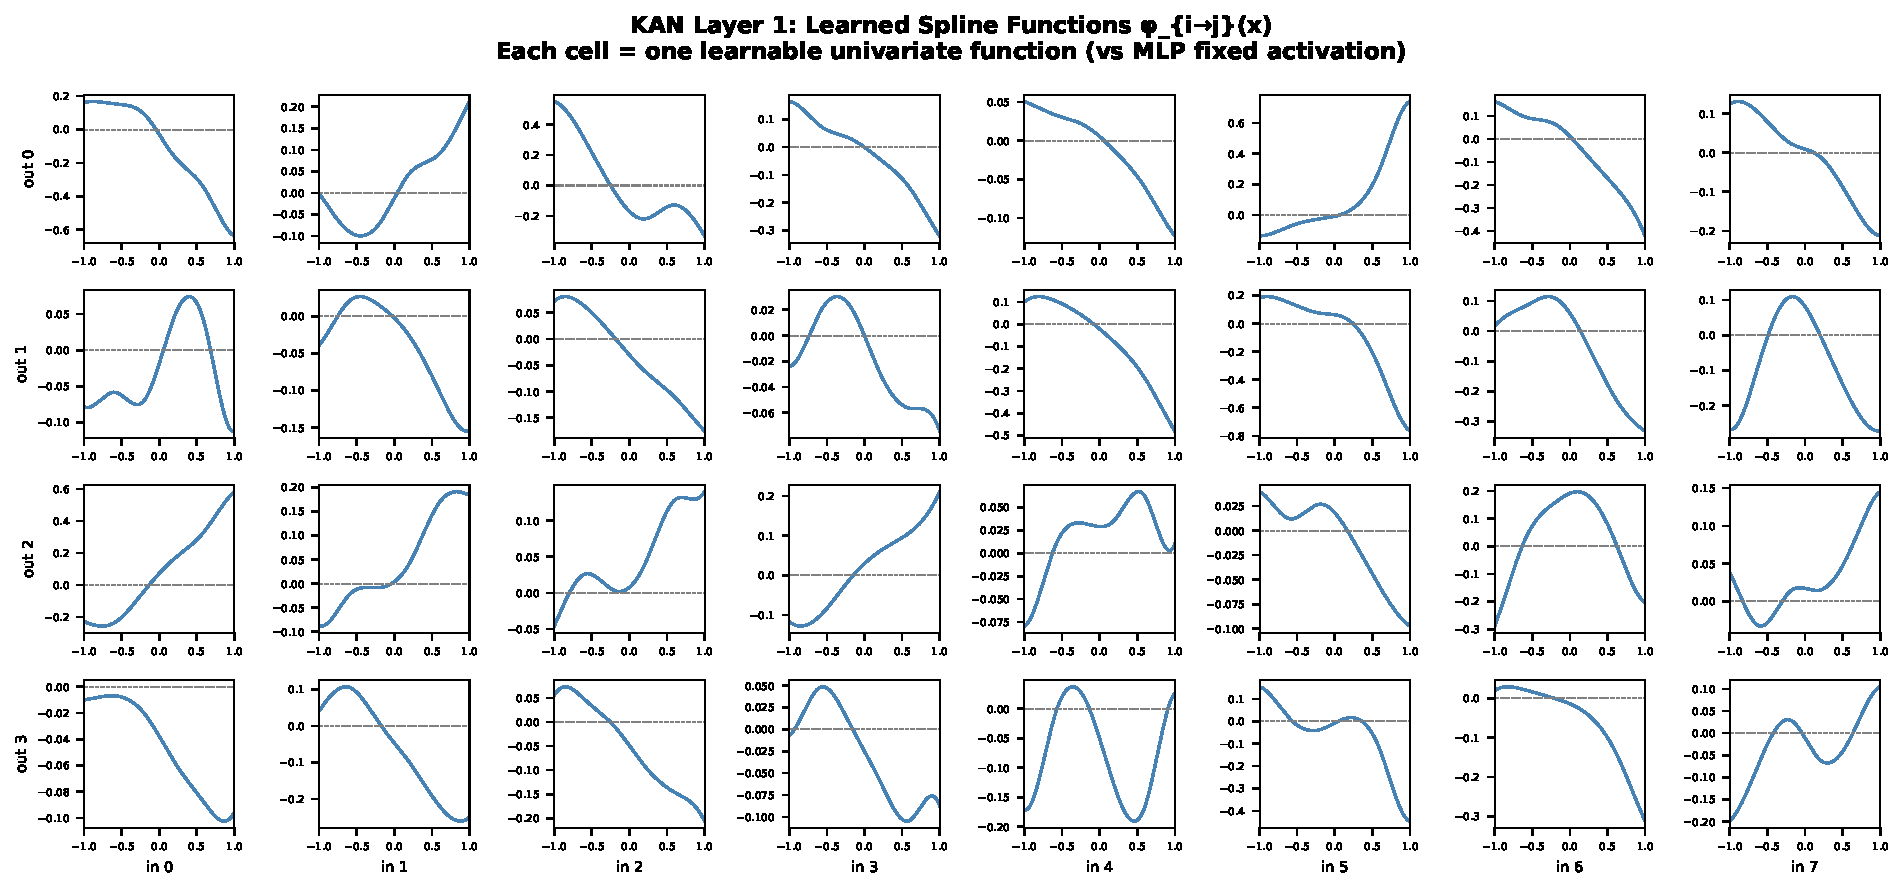
\includegraphics[width=\linewidth]{results/interpretability/fig3_spline_functions.pdf}
    \caption{Spline activations}
  \end{subfigure}
  \hfill
  \begin{subfigure}{0.48\linewidth}
    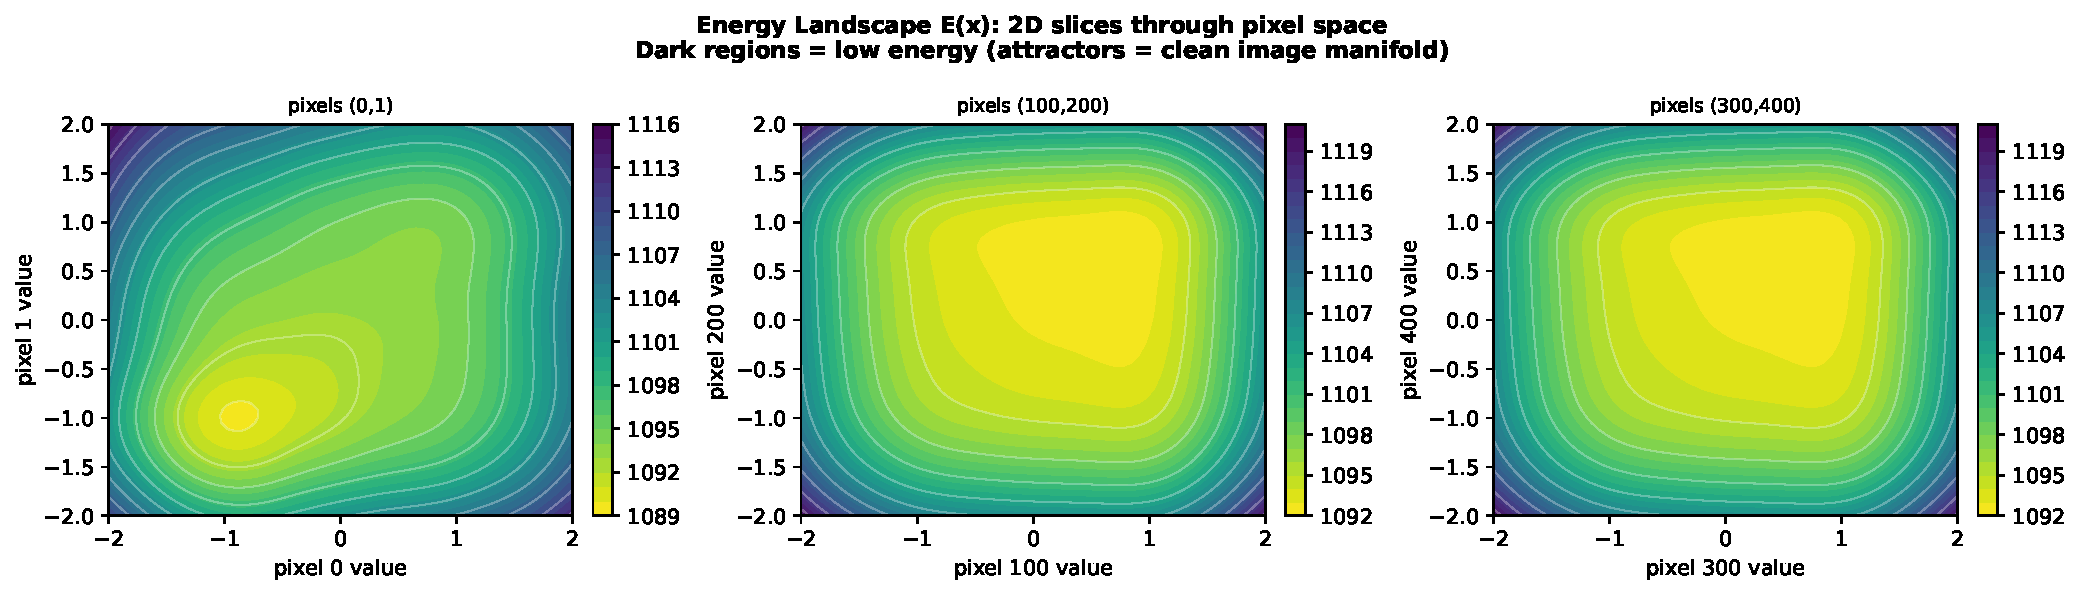
\includegraphics[width=\linewidth]{results/interpretability/fig4_energy_landscape.pdf}
    \caption{Energy basins}
  \end{subfigure}
  \caption{Learned representations: the spline activations span a diverse set of monotone and non-monotone functions; energy basins near clean training images are well-defined.}
  \label{fig:interp}
\end{figure}

\end{document}
